\section{ÔN TẬP CHƯƠNG 2}
\subsection{TRẮC NGHIỆM NHIỀU PHƯƠNG ÁN LỰA CHỌN}
\setcounter{ex}{0}
\Opensolutionfile{ans}[ans/G10Y25B5-TN]
\begin{ex}
	Chọn phát biểu \textbf{sai}. Một vật chuyển động thẳng đều có
	\choice
	{quãng đường vật đi được tỉ lệ với thời gian chuyển động}
	{\True tọa độ của vật tỉ lệ thuận với vận tốc}
	{tọa độ của vật là hàm bậc nhất theo thời gian}
	{độ dịch chuyển tỉ lệ thuận với vận tốc}
	\loigiai{}
\end{ex}

\begin{ex}
	Độ lớn của độ dịch chuyển bằng quãng đường đi được khi vật
	\choice
	{\True chuyển động thẳng và không đổi chiều}
	{chuyển động thẳng có đổi chiều}
	{chuyển động tròn đều quanh một trục}
	{chuyển động theo đường cong bất kỳ}
	\loigiai{}
\end{ex}

\begin{ex}
	Trong trường hợp nào sau đây \textbf{không thể} coi vật chuyển động là chất điểm?
	\choice
	{Ô tô di chuyển từ Đà Nẵng đến Quảng Nam}
	{Viên bi rơi từ tầng năm của một tòa nhà xuống đất}
	{Trái Đất chuyển động quay quanh Mặt Trời}
	{\True Trái Đất tự quay quanh trục của nó}
	\loigiai{}
\end{ex}

\begin{ex}
	Tốc độ là đại lượng đặc trưng cho
	\choice
	{\True tính chất nhanh hay chậm của chuyển động}
	{sự thay đổi hướng của chuyển động}
	{khả năng duy trì chuyển động của vật}
	{sự thay đổi vị trí của vật trong không gian}
	\loigiai{}
\end{ex}

\begin{ex}
	Một người chuyển động thẳng có độ dịch chuyển $d_1$ tại thời điểm $t_1$ và độ dịch chuyển $d_2$ tại thời điểm $t_2$. Vận tốc trung bình của vật trong khoảng thời gian từ $t_1$ đến $t_2$ là
	\choice
	{$v_{tb}=\dfrac{d_1-d_2}{t_1+t_2}$}
	{\True $v_{tb}=\dfrac{d_2-d_1}{t_2-t_1}$}
	{$v_{tb}=\dfrac{d_1+d_2}{t_2-t_1}$}
	{$v_{tb}=\dfrac{1}{2}\left(\dfrac{d_1}{t_1}+\dfrac{d_2}{t_2}\right)$}
	\loigiai{}
\end{ex}

\begin{ex}
	Cho quãng đường $AB$ dài \SI{1000}{\meter} với $A$ là vị trí nhà em, $B$ là bưu điện, $C$ là tiệm tạp hoá nằm ở trung điểm $AB$.  
	Chọn gốc tọa độ tại nhà em và chiều dương hướng từ nhà đến bưu điện.  
	Khi em đi từ nhà đến bưu điện, sau đó đi từ nhà đến tiệm tạp hoá rồi quay lại nhà, quãng đường đi được $s$ và độ dịch chuyển $d$ lần lượt là  
	\begin{center}
		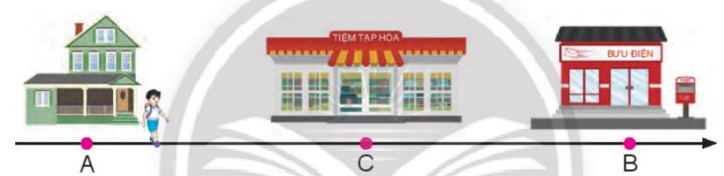
\includegraphics[scale=1.0]{figs/G10Y25B5-15}
	\end{center}
	\choice
	{$s=\SI{500}{\meter},\ d=\SI{500}{\meter}$}
	{\True $s=\SI{1000}{\meter},\ d=\SI{0}{\meter}$}
	{$s=\SI{1000}{\meter},\ d=\SI{500}{\meter}$}
	{$s=\SI{0}{\meter},\ d=\SI{1000}{\meter}$}
	\loigiai{}
\end{ex}

\begin{ex}
	Cặp đồ thị nào dưới đây là của chuyển động thẳng đều?
	\begin{center}
		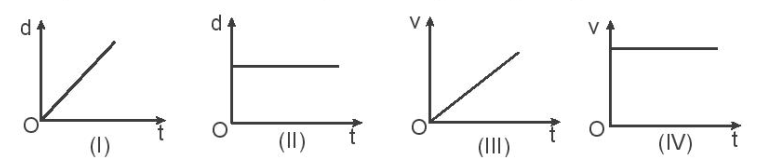
\includegraphics[scale=0.6]{figs/G10Y25B5-2}
	\end{center}
	\choice
	{I và III}
	{\True I và IV}
	{II và III}
	{II và IV}
	\loigiai{}
\end{ex}

\begin{ex}
	Độ dốc của tiếp tuyến với đồ thị $(d\text{–}t)$ tại thời điểm đang xét cho biết điều gì?
	\choice
	{độ lớn gia tốc tức thời của vật tại thời điểm đó}
	{\True tốc độ tức thời của vật tại thời điểm đó}
	{thời điểm vật đổi chiều chuyển động}
	{khoảng cách ban đầu của vật tới gốc tọa độ}
	\loigiai{}
\end{ex}

\begin{ex}
	Trong Vật lí cổ điển, đại lượng nào \textbf{không có} tính tương đối?
	\choice
	{Quỹ đạo}
	{Vận tốc}
	{Tốc độ}
	{\True Khối lượng}
	\loigiai{}
\end{ex}

\begin{ex}
	Hãy thiết lập phương trình chuyển động của một ô tô chuyển động thẳng đều biết. Ô tô chuyển động theo chiều dương với vận tốc $\SI{10}{\meter/\second}$ và ở thời điểm $\SI{3}{\second}$ thì vật có tọa độ $\SI{60}{\meter}$.
	\choice
	{\True $\xsi{30+10t}{\meter}$}
	{$\xsi{20+10t}{\meter}$}
	{$\xsi{10+20t}{\meter}$}
	{$\xsi{40+10t}{\meter}$}
	\loigiai{
		Phương trình chuyển động của ô tô:
		$$x=x_0+\SI{10}{t}$$
		Khi $t=\SI{3}{\second}$ thì vật có toạ độ $x=\SI{60}{\meter}\Rightarrow x_0=\SI{30}{\meter}.$
	}
\end{ex}

\begin{ex}
	Lúc 7 giờ sáng, tại A xe thứ nhất chuyển động thẳng đều với tốc độ $\SI{12}{\kilo\meter/\hour}$ để về B. Một giờ sau, tại B xe thứ hai cũng chuyển động thẳng đều với tốc độ $\SI{48}{\kilo\meter/\hour}$ theo chiều ngược lại để về A. Cho đoạn thẳng $AB=\SI{72}{\kilo\meter}$. Khoảng cách giữa hai xe lúc 10 giờ là
	\choice
	{$\SI{12}{\kilo\meter}$}
	{\True $\SI{60}{\kilo\meter}$}
	{$\SI{36}{\kilo\meter}$}
	{$\SI{24}{\kilo\meter}$}
	\loigiai{
		Chọn gốc toạ độ tại A, chiều dương hướng từ A đến B. Chọn gốc thời gian lúc $\SI{7}{\hour}$.
		Phương trình chuyển động của mỗi xe:
		\begin{align*}
			\begin{cases}
				x_1=\xsi{12t}{\kilo\meter}\\
				x_2=\xsi{72-48(t-1)}{\kilo\meter}
			\end{cases}
		\end{align*}
		Khoảng cách hai xe lúc $\SI{10}{\hour}$, tương ứng $t=\SI{3}{\hour}$:
		$$\Delta x=\left|x_1-x_2\right|=\SI{60}{\kilo\meter}$$
	}
\end{ex}

\begin{ex}
	Một chiếc máy bay đang bay từ Thành phố Hồ Chí Minh đến Thủ đô Hà Nội với tốc độ $\SI{525}{\kilo\meter/\hour}$. Trong hôm đó, gió thổi về hướng Nam với tốc độ $\SI{36}{\kilo\meter/\hour}$. Xem như máy bay chuyển động thẳng đều theo hướng Bắc và quãng đường bay từ Thành phố Hồ Chí Minh đến Thủ đô Hà Nội là $\SI{1160}{\kilo\meter}$. Hãy xác định thời gian bay của máy bay trên quãng đường đó.
	\choice
	{$\SI{3,27}{\hour}$}
	{$\SI{7,32}{\hour}$}
	{$\SI{1,37}{\hour}$}
	{\True $\SI{2,37}{\hour}$}
	\loigiai{
		Gọi:
		$\vec v_{1,2}$ là vận tốc của máy bay so với gió.
		$\vec v_{2,3}$ là vận tốc của gió so với mặt đất.
		$\vec v_{1,3}$ là vận tốc của máy bay so với mặt đất.
		Ta có:
		$$\vec v_{1,3} = \vec v_{1,2} + \vec v_{2,3}.$$
		Tốc độ của máy bay so với gió là $v_{1,2}= \SI{525}{\kilo\meter/\hour}$; tốc độ của gió so với mặt đất là $ v_{2,3}= \SI{36}{\kilo\meter/\hour}$.
		Chọn chiều dương là chiều chuyển động của máy bay (hướng bắc).
		Do gió chuyển động theo hướng nam nên: $v_{2,3} <0$.
		Vận tốc của máy bay:
		$$v_{1,3} = v_{1,2} - v_{2,3} = \SI{489}{\kilo\meter/\hour}.$$
		Thời gian bay của máy bay trên quãng đường $\SI{1160}{\kilo\meter}$ là:
		$$ t =\dfrac{S}{v} \approx \SI{2,37}{\hour}.$$
	}
\end{ex}

\Closesolutionfile{ans}
\subsection{TRẮC NGHIỆM ĐÚNG SAI}
\setcounter{ex}{0}
\Opensolutionfile{ans}[ans/G10Y25B5-TF]
\begin{ex}
	Một robot dọn dẹp được lập trình để di chuyển trên một đường thẳng dọc hành lang. Đồ thị chuyển động của nó được vẽ trên hình bên dưới:
	\begin{center}
		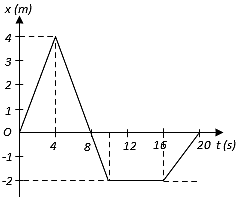
\includegraphics[scale=1]{figs/G10Y25B5-16}
	\end{center}
	\choiceTF[t]
	{\True Robot đứng yên trong giai đoạn từ $\SI{10}{\second}$ đến $\SI{16}{\second}$}
	{Robot chuyển động thẳng đều trong giai đoạn từ $\SI{0}{\second}$ đến $\SI{8}{\second}$}
	{\True Vận tốc tức thời của robot tại thời điểm $\SI{4}{\second}$ là $\SI{-1}{\meter/\second}$}
	{Tốc độ trung bình của robot trong cả quá trình chuyển động là $\SI{0,3}{\meter/\second}$}
	\loigiai{
		\begin{enumerate}[label=\alph*)]
			\item \textbf{Đúng}.  
			\item \textbf{Sai} – tại $t=\SI{4}{\second}$ vận tốc thay đổi nên không thể kết luận thẳng đều trong toàn bộ $\SI{8}{\second}$ đầu.  
			\item \textbf{Đúng} - $v = \frac{\Delta x}{\Delta t}
			= \frac{0 - 4}{8 - 4}
			= -1\;(\si{\meter\per\second})$.  
			\item \textbf{Sai} – $v_{tb} = \frac{s}{t}
			= \frac{4 + 4 + 2 + 2}{20}
			= 0{,}6\;(\si{\meter\per\second})$
	\end{enumerate}}
\end{ex}

\begin{ex}
	Xác định Đúng (Đ) hoặc Sai (S) cho các phát biểu về chuyển động của bạn A từ nhà đến trường theo lộ trình \(ABC\) (Hình vẽ), biết \(AB=\SI{400}{\meter}\) hết 6 phút, \(BC=\SI{300}{\meter}\) hết 4 phút.
	\begin{center}
		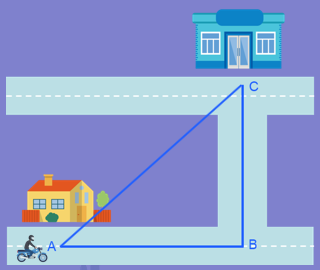
\includegraphics[scale=0.6]{figs/G10Y25B5-17}
	\end{center}
	\choiceTF[t]
	{Độ dài quãng đường từ nhà đến trường là \(\SI{600}{\meter}\)}
	{\True Tốc độ trung bình của bạn A khi đi từ nhà đến trường là \(\approx\SI{1.167}{\meter\per\second}\)}
	{Độ dịch chuyển của bạn A là \(\SI{700}{\meter}\)}
	{\True Vận tốc trung bình của bạn A khi đi từ nhà đến trường là \(\approx\SI{0.83}{\meter\per\second}\)}
	\loigiai{
		\begin{enumerate}[label=\alph*)]
			\item \textbf{Sai}. Quãng đường thực đi \(s=AB+BC=400+300=\SI{700}{\meter}\).
			\item \textbf{Đúng}. Tổng thời gian $t=6+4=10\text{ phút}=600\text{ s}$, nên \(v=\frac{700}{600}\approx\SI{1.167}{\meter\per\second}\).
			\item \textbf{Sai}. Độ dịch chuyển \(d=\sqrt{AB^2+BC^2}=\sqrt{400^2+300^2}=\SI{500}{\meter}\).
			\item \textbf{Đúng}. Vận tốc trung bình \(v=\frac{d}{t}=\frac{500}{600}\approx\SI{0.83}{\meter\per\second}\).
		\end{enumerate}
	}
\end{ex}
\Closesolutionfile{ans}
\subsection{TRẢ LỜI NGẮN}
\setcounter{ex}{0}
\Opensolutionfile{ans}[ans/G10Y25B5-SA]
\begin{ex}
	Trong trận đấu giữa Đức và Áo ở EURO 2008, tiền vệ Michael Ballack của đội tuyển Đức sút phạt cách khung thành của đội Áo $\SI{30}{\meter}$. Các chuyên gia tính được tốc độ trung bình của quả phạt đó lên tới $\SI{108}{\kilo\meter/\hour}$. Hỏi thời gian bay của quả bóng là bao nhiêu giây?
	\shortans[oly]{1}
	\loigiai{
		Thời gian bay của quả bóng:
		$$t=\dfrac{s}{v} = \SI{1}{\second}$$
	}
\end{ex}

\begin{ex}
	Hình \ref{fig:0002-4} mô tả đồ thị độ dịch chuyển - thời gian của một chiếc xe ô tô chạy trên đường thẳng. Tính vận tốc trung bình của xe theo đơn vị $\SI{}{\kilo\meter/\hour}$.
	\begin{center}
		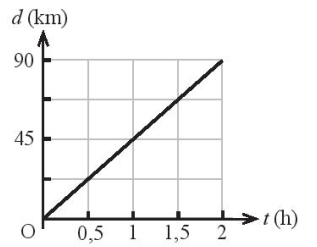
\includegraphics[scale=0.6]{figs/G10Y25B5-7}
		\captionof{figure}{Đồ thị độ dịch chuyển - thời gian của xe}
		\label{fig:0002-4}
	\end{center}
	\shortans[oly]{45}
	\loigiai{
		\text{Vận tốc trung bình của xe}
		$$v=\dfrac{\Delta d}{\Delta t}=\SI{45}{\kilo\meter/\hour}.$$
	}
\end{ex}

\begin{ex}
	Một chiếc ô tô chạy từ điểm A đến điểm B. Nửa quãng thời gian đầu ô tô đi với tốc độ $v_1=\SI{40}{\kilo\meter/\hour}$. Trong quãng thời gian còn lại thì một nửa quãng thời gian đầu ô tô đi với tốc độ $v_2=\SI{50}{\kilo\meter/\hour}$, một nửa quãng thời gian cuối ô tô đi với tốc độ $v_3=\SI{60}{\kilo\meter/\hour}$. Tính tốc độ trung bình của ô tô trên cả đoạn đường AB theo đơn vị $\SI{}{\kilo\meter/\hour}$.
	\shortans[oly]{47,3}
	\loigiai{
		\begin{center}
			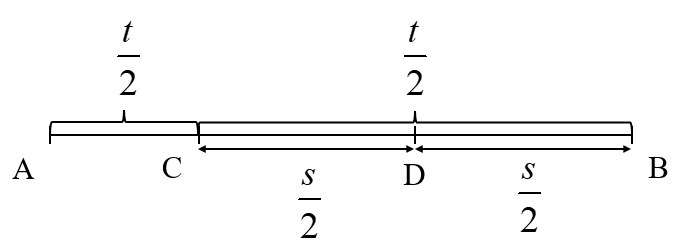
\includegraphics[scale=0.5]{figs/G10Y25B5-14}
		\end{center}
		\text{Xét đoạn CB:}\\
		\text{Tốc độ trung bình:}
		\[
		v_{CB}
		=\frac{CB}{t_{CB}}
		=\frac{CB}{\frac{CD}{v_1}+\frac{DB}{v_2}}
		=\frac{s}{\frac{s/2}{v_1}+\frac{s/2}{v_2}}
		=\frac{1}{\tfrac12\Bigl(\frac1{v_1}+\frac1{v_2}\Bigr)}
		=\frac{1}{\tfrac12\bigl(\tfrac1{50}+\tfrac1{60}\bigr)}
		=\frac{600}{11}\;(\si{\kilo\meter/\hour}).
		\]
		
		\text{Xét đoạn AB:}\\
		\text{Tốc độ trung bình:}
		\[
		v_{tb}
		=\frac{AB}{t_{AB}}
		=\frac{AC+CB}{t}
		=\frac{v_1\frac t2 + v_{CB}\frac t2}{t}
		=\frac{v_1+v_{CB}}{2}
		=\frac{40+\tfrac{600}{11}}{2}
		\approx 47{,}3\;(\si{\kilo\meter/\hour}).
		\]
	}
\end{ex}

\begin{ex}
	Một ô tô đang chạy với vận tốc $v$ theo phương nằm ngang thì người ngồi trong xe trông thấy giọt mưa rơi tạo thành những vạch làm với phương thẳng đứng một góc $\SI{45}{\degree}$. Biết tốc độ của các giọt mưa so với mặt đất là $\SI{5}{\meter/\second}$. Xác định vận tốc của ô tô theo đơn vị $\SI{}{\meter/\second}$.
	\shortans[oly]{5}
	\loigiai{
		\text{Gọi:}
		\begin{itemize}
			\item (1) \text{là giọt mưa};
			\item (2) \text{là xe};
			\item (3) \text{là mặt đường}.
		\end{itemize}
		\text{Vận tốc của giọt mưa so với xe:}
		$$\vec v_{12}=\vec v_{13}-\vec v_{23}$$
		\begin{center}
			\begin{tikzpicture}
				\coordinate (O) at (0,0);
				\coordinate (B) at (4,0);
				\coordinate (C) at (-4,0);
				\coordinate (D) at (0,4);
				\tkzMarkRightAngle[size=0.3,color=cyan](D,O,C);
				\foreach \i in {O}{
					\filldraw[black] (\i) circle (0.05);
				}
				\draw[-stealth,thick, red] (D) -- (O);
				\draw[-stealth,thick, blue] (O) -- (B);
				\draw[-stealth,thick, blue] (O) -- (C);
				\draw[-stealth,thick] (D) -- (C);
				\node[label={[red,below right]90:$\vec v_{13}$}] at (0,2){};	
				\node[label={[blue,below]90:$\vec v_{23}$}] at (2,-0.25){};	
				\node[label={[blue,below]90:$-\vec v_{23}$}] at (-2,-0.25){};	
				\node[label={[black,left]90:$\vec v_{12}$}] at (-2,2){};
				\tkzMarkAngle[size=0.6,color=black](C,D,O);
				\tkzLabelAngle[color=black,pos=1.2](C,D,O){$\SI{45}{\degree}$}
				
			\end{tikzpicture}
		\end{center}
		\text{Độ lớn vận tốc của ô tô (so với mặt đường):}
		$$v_{23}=v_{13} \tan\SI{45}{\degree}=\SI{5}{\meter/\second}$$
		\text{Vận tốc của ô tô có độ lớn } $\SI{5}{\meter/\second}$.
	}
\end{ex}

\Closesolutionfile{ans}
\subsection{TỰ LUẬN}
\setcounter{ex}{0}
\Opensolutionfile{ans}[ans/G10Y25B5-TL]
\begin{ex}
	Lúc 7~h~15, một người đi xe máy khởi hành từ \(A\) với vận tốc không đổi \(\SI{36}{\kilo\meter/\hour}\) để đuổi theo một người đi xe đạp đã đi được \SI{36}{\kilo\meter}\ từ \(A\), chuyển động với \(\SI{5}{\meter/\second}\). Hỏi hai người gặp nhau lúc mấy giờ?
	\loigiai{
		\textbf{Chọn hệ tọa độ và gốc thời gian:} chiều dương là chiều chuyển động, gốc tọa độ tại \(A\), gốc thời gian \(t=0\) ứng với 7~h~15.  
		
		\textbf{Phương trình chuyển động thẳng:} \(x(t)=x_0+v\,t\).  
		
		\emph{Xe máy:} tại \(t=0\), \(x_m(0)=0\), \(v_m=\SI{36}{\kilo\meter/\hour}\), nên
		\[
		x_m(t)=36\,t.
		\]
		
		\emph{Xe đạp:} tại \(t=0\), \(x_d(0)=36\) km, \(v_d=\SI{5}{\meter/\second}=\SI{18}{\kilo\meter/\hour}\) , nên
		\[
		x_d(t)=36+18\,t.
		\]
		
		\textbf{Gặp nhau khi} \(x_m(t)=x_d(t)\):
		\[
		36\,t=36+18\,t
		\quad\Longrightarrow\quad
		18\,t=36
		\quad\Longrightarrow\quad
		t=2\ (\text{giờ}).
		\]
		Vậy họ gặp nhau lúc 
		\[
		7\text{h}15 + 2\text{h} = \boxed{9\text{h}15}.
		\]
	}
\end{ex}

\begin{ex}
	Hình \ref{fig:0002-3} mô tả đồ thị toạ độ - thời gian của hai xe, hãy nêu đặc điểm chuyển động của mỗi xe.
	\begin{center}
		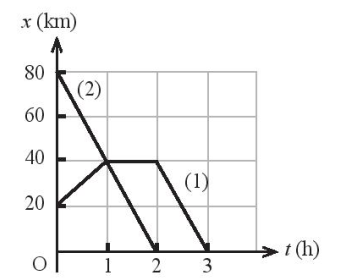
\includegraphics[scale=0.5]{figs/G10Y25B5-6}
		\captionof{figure}{Đồ thị toạ độ - thời gian của hai xe}
		\label{fig:0002-3}
	\end{center}
	\loigiai{
		\begin{itemize}
			\item \text{Chuyển động của xe 1:}
			\begin{itemize}
				\item \text{Trong khoảng thời gian từ } $\SI{0}{\hour}$ \text{đến } $\SI{1}{\hour}$, \text{xe chuyển động đều theo chiều dương với tốc độ } $\SI{20}{\kilo\meter/\hour}$.
				\item \text{Trong khoảng thời gian từ } $\SI{1}{\hour}$ \text{đến } $\SI{2}{\hour}$, \text{xe đứng yên}.
				\item \text{Trong khoảng thời gian từ } $\SI{2}{\hour}$ \text{đến } $\SI{3}{\hour}$, \text{xe chuyển động đều theo chiều âm với tốc độ } $\SI{40}{\kilo\meter/\hour}$.
			\end{itemize}
			\item \text{Chuyển động của xe 2: Trong khoảng thời gian từ } $\SI{0}{\hour}$ \text{đến } $\SI{2}{\hour}$, \text{xe chuyển động đều theo chiều âm với tốc độ } $\SI{40}{\kilo\meter/\hour}$
		\end{itemize}
	}
\end{ex}

\begin{ex}
	Một ca nô chạy ngang qua một dòng sông, xuất phát từ A, hướng mũi về B. Sau $\SI{100}{\second}$, ca nô cập bờ bên kia ở điểm C cách B $\SI{200}{\meter}$. Nếu người lái hướng mũi ca nô theo hướng AD và vẫn giữ tốc độ máy như cũ thì ca nô sẽ cập bờ bên kia tại đúng điểm B. Tìm
	\begin{center}
		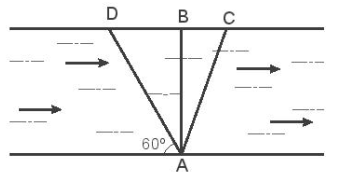
\includegraphics[scale=0.7]{figs/G10Y25B5-10}
	\end{center}
	\begin{enumerate}[label=\alph*)]
		\item Vận tốc của dòng nước so với bờ sông.
		\item Vận tốc của ca nô so với dòng nước.
		\item Chiều rộng của sông.
	\end{enumerate}
	\loigiai{
		\begin{enumerate}[label=\alph*)]
			\item \text{Gọi:}
			\begin{itemize}
				\item $\vec v_{12}$ \text{là vận tốc của ca nô so với dòng nước};
				\item $\vec v_{23}$ \text{là vận tốc của dòng nước so với bờ sông};
				\item $\vec v_{13}$ \text{là vận tốc của ca nô so với bờ sông}.
			\end{itemize}
			\begin{center}
				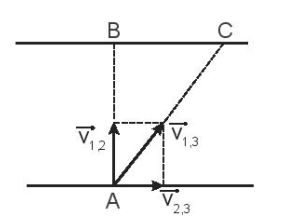
\includegraphics[scale=0.3]{figs/G10Y25B5-11}
			\end{center}
			\text{Khi mũi ca nô hướng về B thì}
			$$\vec v_{13}=\vec v_{12}+\vec v_{23}$$
			\text{với } $v_{12}=\dfrac{AB}{t}$ \text{và } $v_{23}=\dfrac{BC}{t}=\dfrac{\SI{200}{\meter}}{\SI{100}{\second}}=\SI{2}{\meter/\second}$.\\
			\item \text{Khi mũi ca nô hướng về D thì }
			\begin{center}
				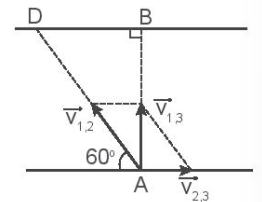
\includegraphics[scale=0.5]{figs/G10Y25B5-13}
			\end{center}
			$$\overrightarrow v'_{13}=\overrightarrow v'_{12}+\overrightarrow v'_{23}$$
			\text{với } $v'_{12}=v_{12}$ \text{và } $v'_{23}=v_{23}=\SI{2}{\meter/\second}$.\\
			\text{Ta có:}
			$$v'_{12}=\dfrac{v'_{12}}{\sin\SI{30}{\degree}}=\SI{4}{\meter/\second}$$
			\item $AB=v_{12}\cdot t=\SI{400}{\meter}$.
		\end{enumerate}
	}
\end{ex}
\Closesolutionfile{ans}